\section{System Design and Implementation}

\begin{figure}[tbh]
    \centering
    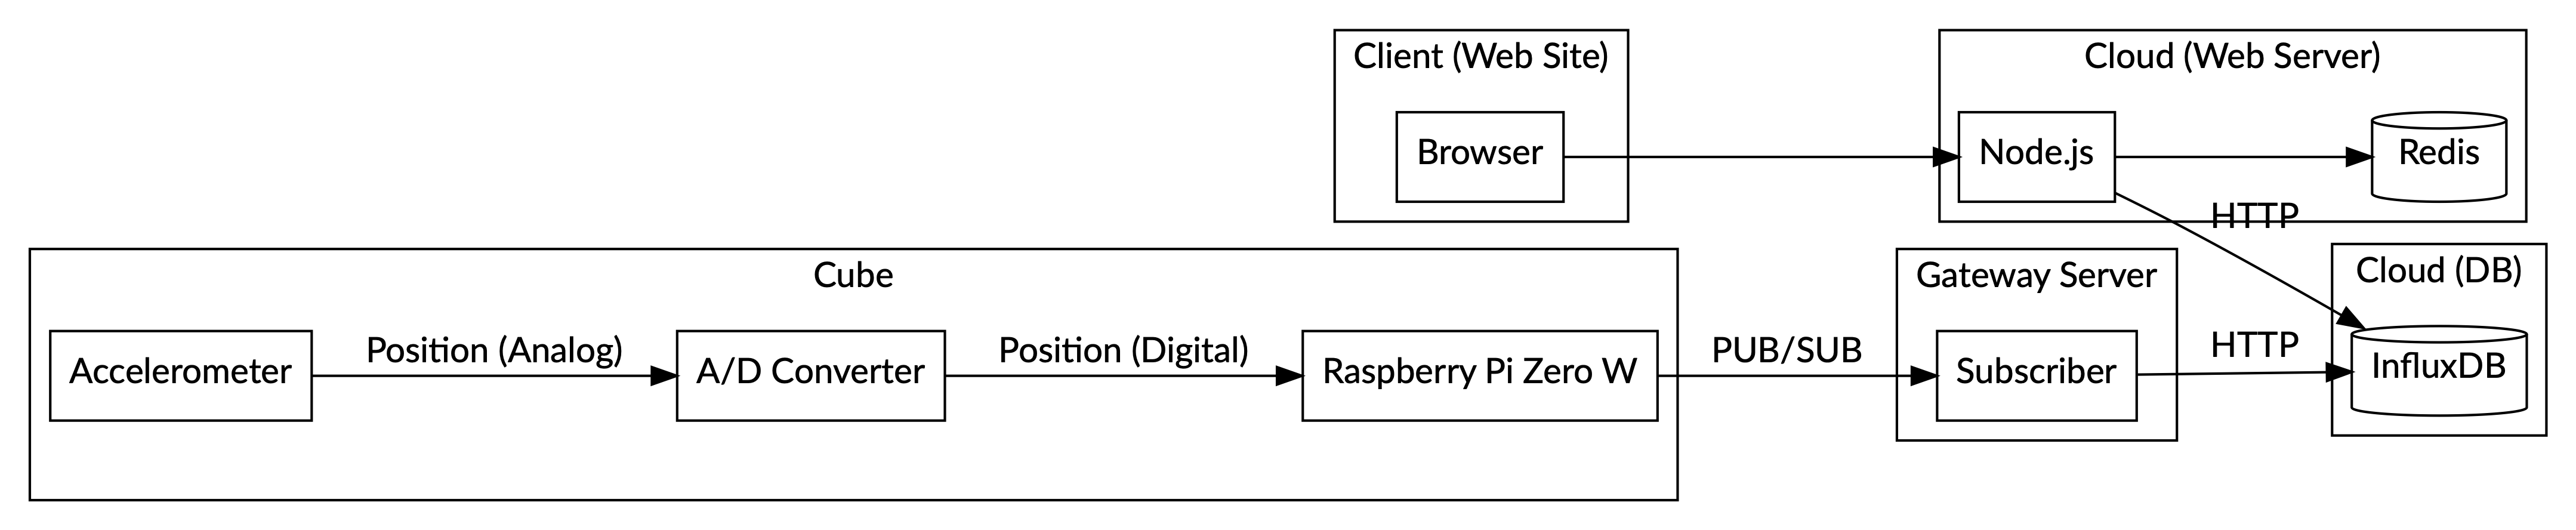
\includegraphics[width=\linewidth]{architecture.png}
    \caption{The overall system architecture of the TimeCube system.}
    \label{fig:architecture}
\end{figure}

\subsection{System Overview}

The TimeCube is a distributed system. The actual cube is a wooden construction containing a Raspberry Pi Zero W, an accelerometer, and an A/D converter. This part of the setup is responsible for figuring out which side of the cube is facing the top, and to provide a facility to publish that information to the outside world.

A gateway server is used to gather that information from one or multiple cubes, which can be distinguished by an identifier published with the side indication. The data is collected and forwarded in order to be stored in a database. The gateway's role is to connect the local network to the world wide web.

The actual database ‒ an InfluxDB time series database ‒ is located in the cloud. The data from one or many gateways, which could be connected to one or multiple cubes, is collected in a single database. The devices are distinguished by a UUID, which is reported alongside the cube's top-facing side.

A web site for configuration (the cube's side's meaning) and reporting (tabular and visualized as a bar plot) is provided on a web server. Conceptually, the web and gateway server are two distinct entities, but can be run on the same physical server.

A detailed system architecture is shown on \imgref{fig:architecture}.

\subsection{Software Components}

The \texttt{timecube} component figures out the top-facing side of the cube and publishes that information, alongside a UUID to identify the device, to the gateway server. The \texttt{sub\_influx} component subscribes to the data streams of multiple TimeCube devices, and forwards the data points to an InfluxDB instance running in the cloud.

A web application is used for reporting. It consists of two components: First, the \texttt{web\_\-back\-end} component deals with persistent data. It offers HTTP endpoints for storing and receiving configuration data (the value of the cube's six sides) and transaction data (the activities reported by the individual devices). Second, the \texttt{web\_frontend} component offers a web interface to configure the cube's six sides individually, and create reports for a specific time frame. The activities are reported in a table (list of activities with start and end date, duration, and the name of the respective activity in respect to the configuration) and as a bar chart, which reports the total duration of the six configured activities.

The \texttt{timecube} and \texttt{sub\_influx} components are implemented in Python. The \texttt{Adafruit\_\-ADS1x15} library is used to interpret the signals from the A/D converter. A ZeroMQ publish/subscribe socket \cite[p. 245-247]{hintjens2013zeromq} is used for the communication between the TimeCube and the gateway server.

The \texttt{web\_backend} and \texttt{web\_frontend} components are both implemented in JavaScript. Node.js with the Express.js framework is used on the backend. The frontend uses plain JavaScript and D3.js for the plot. The web application can be built and run using Docker Compose.\footnote{See the \texttt{README.md} file in the root directory of the repository for further instructions.}

\subsection{Hardware Components}

The analog signal of the accelerometer is converted to a digital signal using an A/D converter. An I²C (Inter-Integrated Circuit) connection is used between the A/D converter and the Raspberry Pi Zero W. These components are wired together as follows:

\begin{multicols}{2}
    \begin{enumerate}
        \item Raspi (3V3) → Accelerometer (Vin)
        \item Raspi (GND) ← Accelerometer (GND)
        \item Accelerometer (Xout) → A/D Converter (A0)
        \item Accelerometer (Yout) → A/D Converter (A1)
        \item Accelerometer (Zout) → A/D Converter (A2)
        \item Raspi (3V3) → A/D Converter (VDD)
        \item Raspi (GND) ← Accelerometer (GND)
        \item Raspi (SCL) ↔ A/D Converter (SCL)
        \item Raspi (SCA) ↔ A/D Converter (SCA)
    \end{enumerate}
\end{multicols}

The physical wiring of the two prototypes is shown on \imgref{fig:timecube1} (Prototype I) and \imgref{fig:timecube2} (Prototype II).

\begin{figure}
    \centering
    \begin{subfigure}{0.4\textwidth}
        \centering
        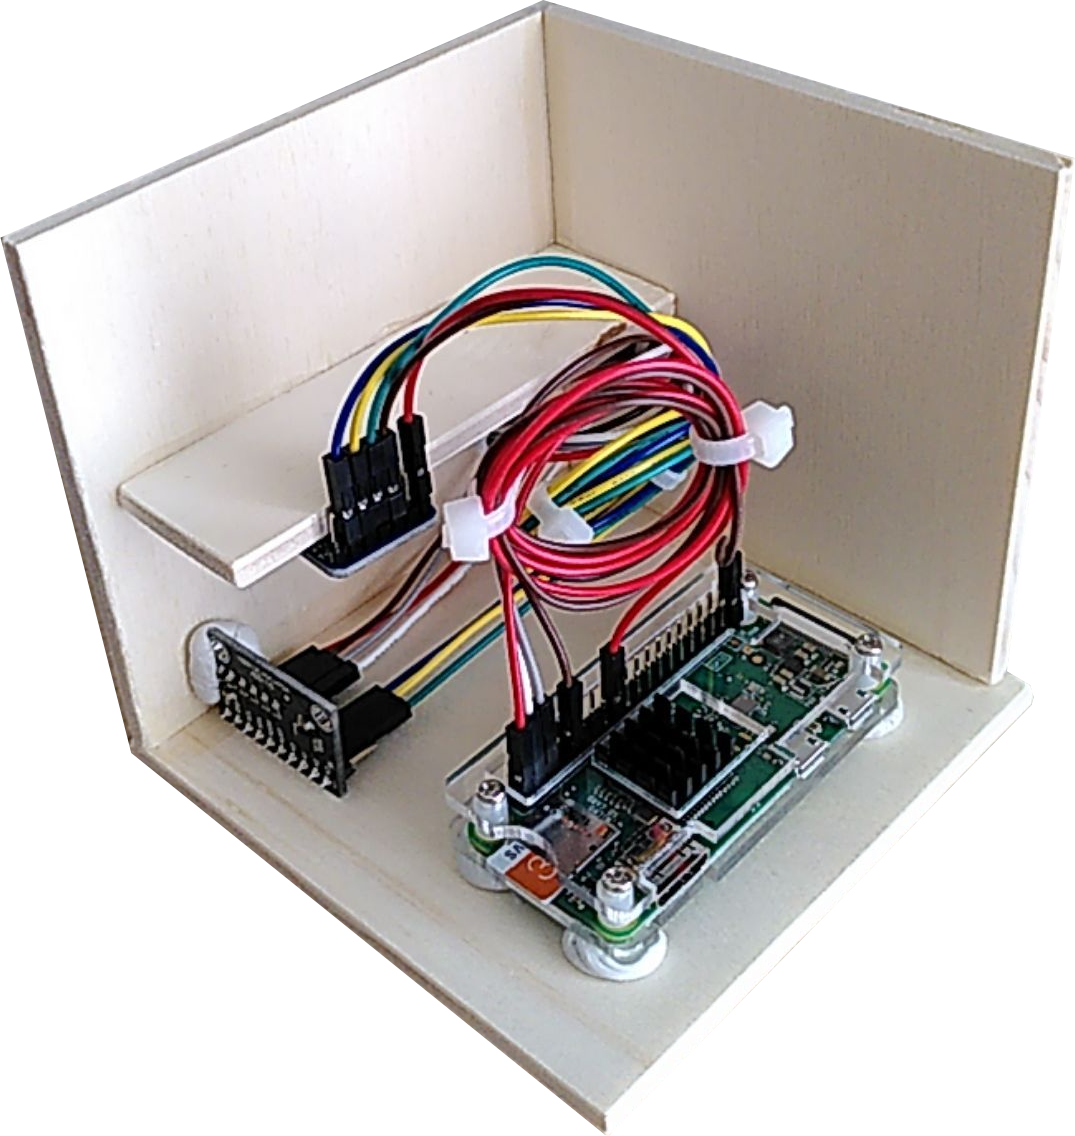
\includegraphics[width=0.95\linewidth]{timecube.png}
        \subcaption{Prototype I}
        \label{fig:timecube1}
    \end{subfigure}
    \begin{subfigure}{0.4\textwidth}
        \centering
        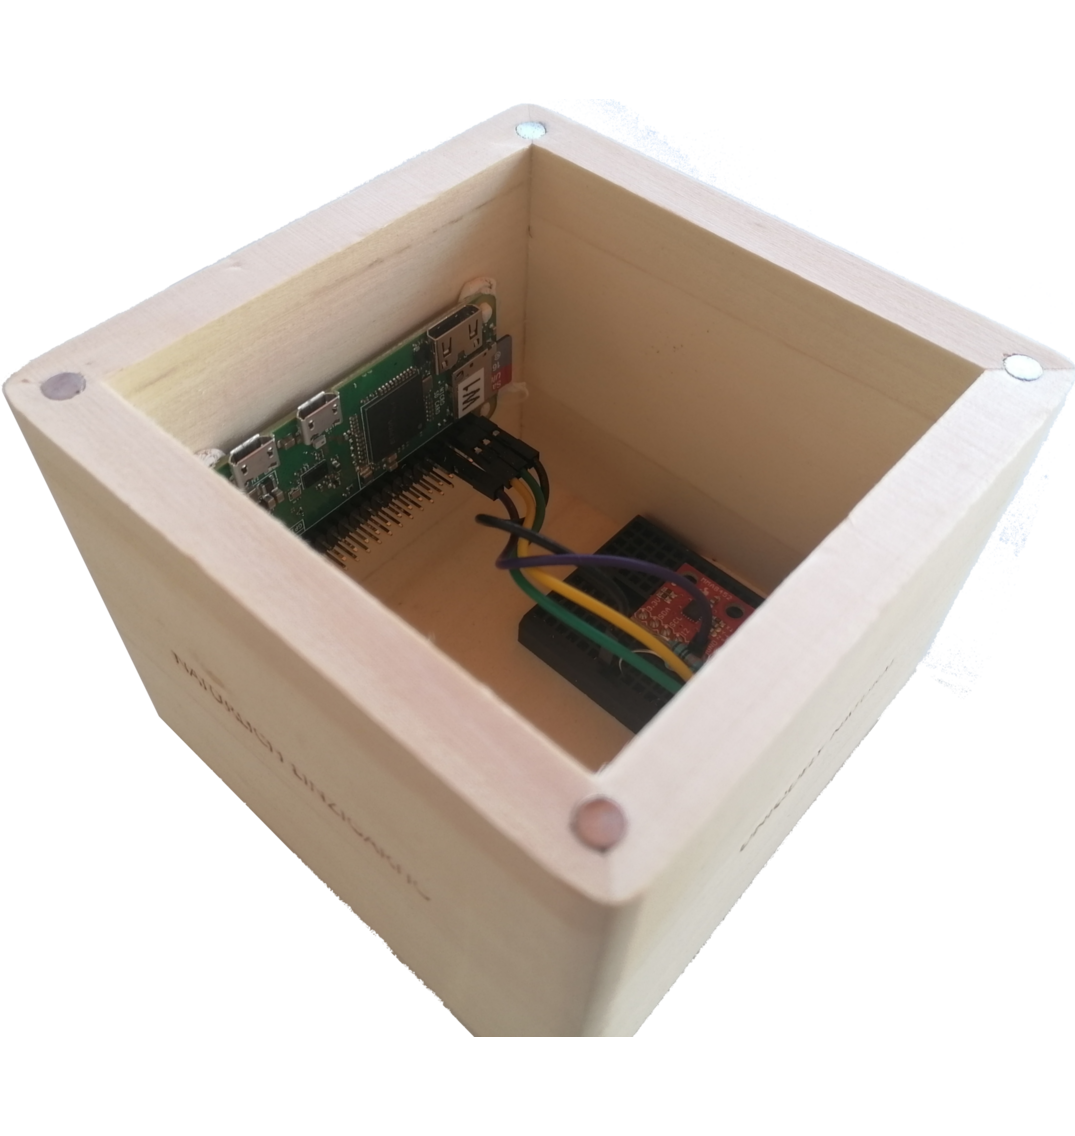
\includegraphics[width=0.95\linewidth]{timecube2.png}
        \subcaption{Prototype II}
        \label{fig:timecube2}
    \end{subfigure}
    \caption{The wooden TimeCube prototypes, containing a Raspberry Pi Zero W, an accelerometer, and an A/D converter, wired together.}
\end{figure}
